\section{Results}
\label{sec:chap_slam_results}

In this section, we first explain how we produced the results data and discuss about some general observations about the results for our three datasets. We then analyse the results between the unstructured and structured environments as well as between the SICK and the Velodyne acquisitions. 

\subsection{Data and General Observations}
\label{ssec:chap_slam_performance_evaluation}

In order to evaluate the place recognition performance, two elements are required. Firstly, a rule for labeling two positions of the real world as belonging (or not) to the same place, and secondly, the algorithm prediction for two input scans. In the following subsection, we will first discuss these two elements and present the resulting data. Afterwards, we will explain some observations about those data.


\subsubsection{Real World Places}
The notion of a place can be variable, but the closer two points of the space are to each other, the more likely they are to be considered in the same place. Therefore, we use the real world physical distance between two acquisitions as an indicator of the likelihood that they represent the same place. We will now discuss the method used to determine the distance between scans. 

We first used the robot odometry as a rough approximation of the relative pose between two subsequent scans. In order to reduce the pose estimation error, we then used the \gls*{icp} algorithm to align the two point clouds and adjust the odometry accordingly. These steps were performed sequentially for all scans of the first loop. This technique could not be independently repeated for the second loop, because the difference in error accumulation would cause a discrepancy between the resulting path of the two loops. To address this problem, the \gls*{icp} odometry adjustment of the second loop was performed relative to the first loop. To do this, we first align the first scan of the second loop relative to the first scan of the first loop using \gls*{icp}. Thereafter, each scan of the second loop was adjusted with respect to the scan of the first loop theoretically being closest, considering the last corrected pose and the movement of the robot. Figure~\ref{fig:chap_slam_results_paths} illustrates the resulting paths, as well as the position of each scans of our three datasets. Note that this is a \gls*{2d} representation for which the vertical component was ignored. This figure shows the absence of discrepancy between the two loops of each dataset.

With the corrected odometry it is possible to easily obtain the distance between two scans. To do this, one can simply calculate the norm of the difference in position between the two scans. On the other hand, given the accumulated odometry error, the relative position between the last scan of a loop $L_i$ and the first scan of a loop $L_j$ (including $i=j$) can be significant. The relative error generally also increases over time (with each move to a new acquisition). To reduce the impact of these problems, we used \gls*{icp} to determine the relative pose for all pair \textit{($L_i$ last scan, $L_j$ first scan)}. With these relative poses, it was possible to create the reverse sequential path between two scans. Finally, we use the path for which the scans are closest in terms of acquisition numbers (sequential or reverse) for the final calculation of the distance.

Note that all alignments have been visually inspected to ensure that \gls*{icp} had indeed converged to a valid solution. When this was not the case, the odometry provided by the robot was manually adjusted to enable this convergence. The second line of Figure~\ref{fig:chap_slam_results} show the resulting distances matrices for all pair of scans of each of our three datasets. Note that a distance function is by definition symmetrical, therefore producing a symmetrical matrix. The values on the main diagonal represent the distance between a scan and itself and are therefore null. A secondary diagonal of low values is produced by the small distances between the scans of the first and the second loop. Finally, because we tried to stop the loop acquisitions approximately at the starting point, we observe small values at those junction points (at the bottom left corner for instance).

\begin{figure}[H]
    \centering
    \subfloat[]{\label{fig:building_paths}}{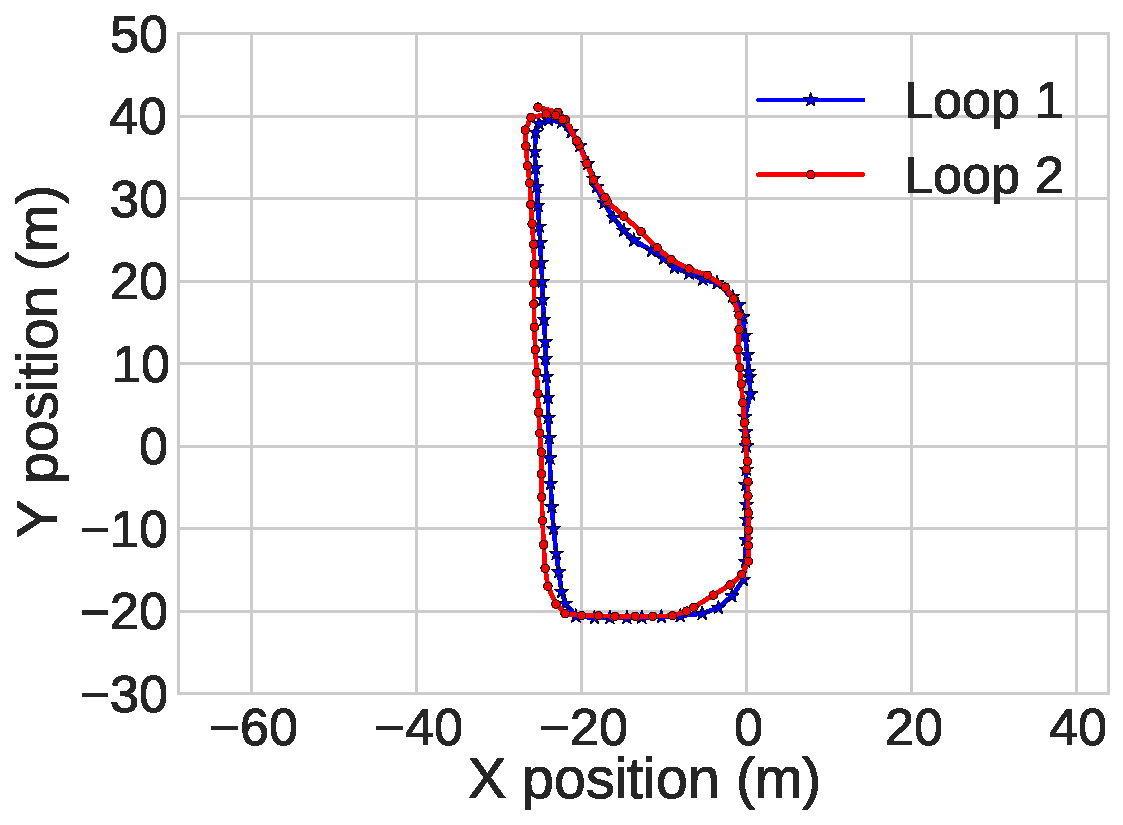
\includegraphics[width=0.45\linewidth]{img/chap_slam/building_paths.pdf}}
    \subfloat[]{\label{fig:forest_paths}}{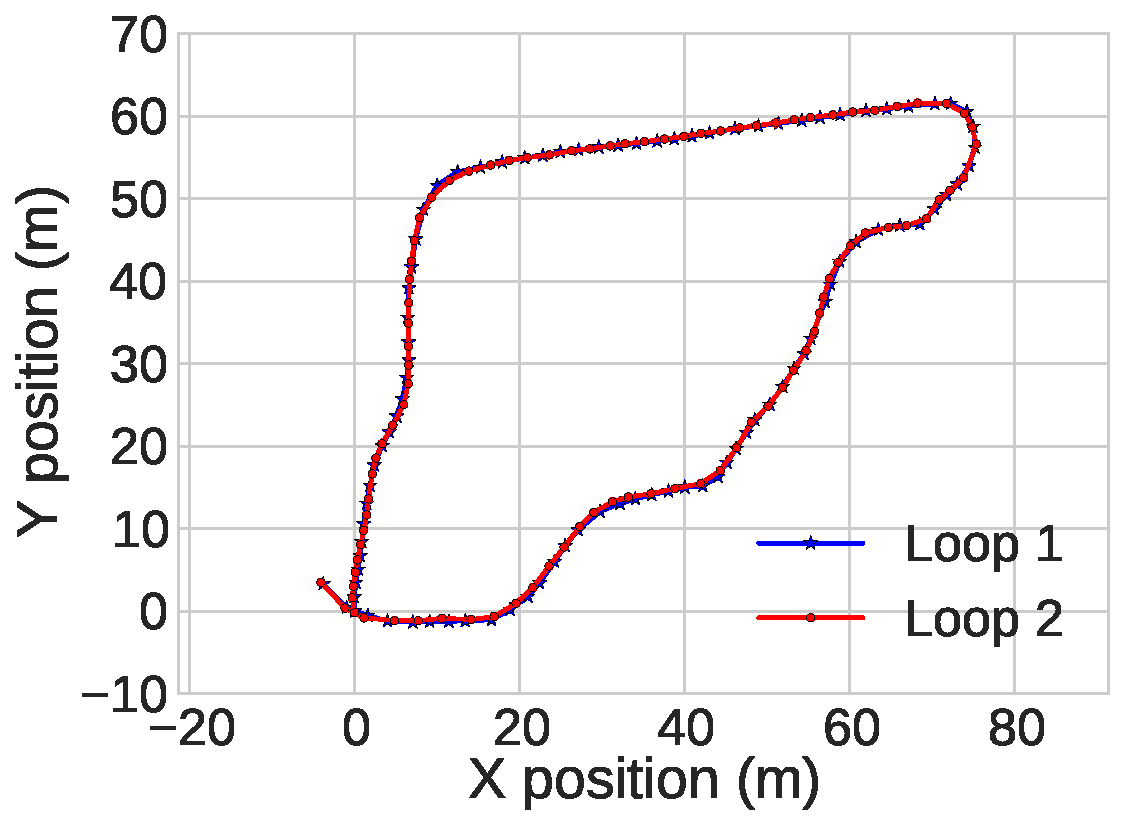
\includegraphics[width=0.45\linewidth]{img/chap_slam/forest_paths.pdf}}
    \subfloat[]{\label{fig:velodyne_paths}}{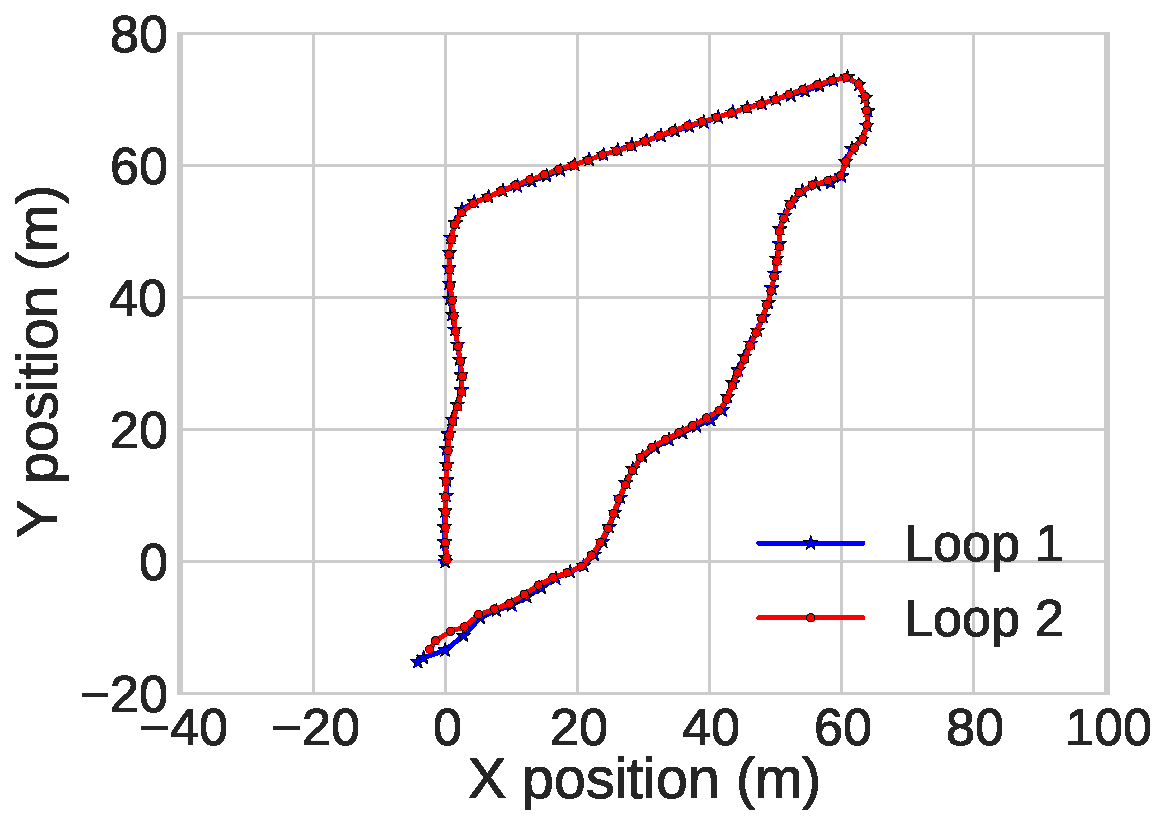
\includegraphics[width=0.45\linewidth]{img/chap_slam/velodyne_paths.pdf}}
    \caption[Path adjusted using \gls*{icp} for our three datasets.]{The path resulting from the odometry adjusted with \gls*{icp} for the two loops of each of our three datasets. \protect\subref{fig:building_paths} shows the path for the Structured-SICK dataset, \protect\subref{fig:forest_paths} shows the path for the Unstructured-SICK dataset and \protect\subref{fig:velodyne_paths} shows the path for the Unstructured-Velodyne dataset. Note that each marker represent the location of an acquisition.}
    \label{fig:chap_slam_results_paths}
\end{figure}


\subsubsection{Algorithm Prediction}
For our experiments, we used a \textit{C++} implementation of the place recognition algorithm developed by Bastian Steder, who provided us the source code. The software, resulting from the compilation of this code, allowed us to obtain a score between 0~and~1 for each pair of scan in the database. As explained in Section~\ref{sec:chap_slam_algo}, this score reflects the system belief that the two scans represents the same place. More precisely, when the score is zero, the algorithm believes there is no chance that the scans originate from the same place, and when the score is one, the algorithm is certain that they do not originate from the same place.

The second row of Figure~\ref{fig:chap_slam_results} represents the scores matrices for our three datasets. Note that the main diagonal of these matrices is the score of a scan compared to itself, which always results in a value of~1. It is possible to observe a slight asymmetry in the matrices caused by the non-symmetric function used for calculating scores. Note that, for our results analysis, we will only consider the values from the area below the main diagonal.


\subsubsection{General Observations}
\label{ssec:chap_slam_results_evaluation}

Considering the two previous subsections, we should expect to see a high score for a pair of close scans and a low score for a pair of remote scans. This relationship can actually be observed by comparing the distances matrices and the scores matrices (first and second rows of Figure~\ref{fig:chap_slam_results}). The third row of Figure~\ref{fig:chap_slam_results} also illustrates this relation by a scatter plot, where each pair of scans is represented by a data point based on the distance between the scans and the score produced by the place recognition algorithm. The set of data points seem to follow a function of the form $f(x) = 1 / x$, which also confirm our prediction.

While it is interesting to observe the relationship between these values over the entire spectrum, practical uses of place recognition generally require a binary labeling of each pair of scans (either originating from the same place or not). To determine the ground truth labels (real world places), a threshold will be defined on the distance between the scans. All pairs of scans closer than this distance threshold will be considered as being in the same place. We will refer to this distance threshold as the place recognition range. Regarding the algorithm prediction labels, a threshold will be set on the output score. All pair of scans obtaining a score higher than this threshold will be labeled as originating from the same place. Table~\ref{tab:chap_slam_results_labeling} summarises how these two thresholds will be used to label data and analyse results.

\begin{table}[H]
    \centering
    \begin{tabular}{@{}l|ll@{}}
        \toprule
                                  & \textbf{$D < T_{distance}$} & \textbf{$D >= T_{distance}$} \\
        \hline
        \textbf{$S > T_{score}$}  & True Positive (TP)          & False Positive (FP) \\
        \textbf{$S <= T_{score}$} & False Negative (FN)         & True Negative (TN) \\
        \bottomrule
    \end{tabular}
    \caption[Summary of scans pairs labeling for results analysis.]{A summary of scans pairs labeling for results analysis. $D$ represents the distance between the two scans and $S$ represents the place recognition algorithm output score. $T_{distance}$ and $T_{score}$ represent the place recognition range and the score threshold, respectively.}
    \label{tab:chap_slam_results_labeling}
\end{table}

As indicated in the introduction of this chapter (Section~\ref{sec:chap_slam_intro}), \gls*{slam} algorithms often use place recognition to detect loop closures. When the robot detects that it is in a place visited before, it can connect (or merge) these concordant regions and adjust the map accordingly. If two scans are falsely identified as coming from the same place (i.e. a false positive), the \gls*{slam} algorithm will distort the map while trying to connect them. In contrast, if a place is not recognized (i.e. false negative), the algorithm simply does not benefit from this cue to adjust the map. Therefore, false positives are more harmful than false negatives and must be avoided. This can be achieve by choosing a score threshold that is high enough, for which the minimum value is depicted by the line in the graphs of the third row of Figure~\ref{fig:chap_slam_results}. Moreover, the closer the value is from that line, the better the recall will be. In our case, the recall represent the fraction of real world places that are correctly identified by the algorithm (i.e. $TP/(TP+FN)$). The recall is presented as function of the place recognition range for different score thresholds in the fourth row of Figure~\ref{fig:chap_slam_results}. One can actually observe that when the score threshold decreases, the recall increases.

Regarding the place recognition range, the desired value will depend on the user's needs, but the higher this value is, the further the robot can be from the previously visited place and still be able to recognize it. Consequently, a higher place recognition range is generally preferable, because it allows greater flexibility during the robot navigation. On the other hand, the further two scans are acquired from each other, the smaller the possible overlap between them is. Note that the structure of the environment can also reduce the overlap between the scans by occluding some regions. This reduction in the overlap between scans result in a decrease of the algorithm output score. The fourth row of Figure~\ref{fig:chap_slam_results} shows how the recall decreases as the place recognition range increases.

\subsection{Comparative Analysis}
\label{ssec:chap_slam_comparative_analysis}

In the previous subsection, we explained how we produced the results and we discuss some observations for our datasets from a general perspective. We will now focus on the main interest of this document and analyze how the algorithm behaves in the unstructured environment compared to the structured environment. We will also conduct this comparative analysis between two \gls*{lidar}s, the SICK LMS151 and the Velodyne HDL-32E. For these comparisons, we will consider how the score changes as function of the place recognition range and look for outliers. Finally, even if the current experimental configuration does not allow to determine the exact source of the result differences, we will suggest some possible causes.


\subsubsection{Structured and Unstructured Environments}
\label{ssec:chap_slam_struct_vs_forest}

For this comparison, we expect the performance of the algorithm to be worse for the unstructured environment than for the structured environment. Our belief is mainly du to the complexity . In order to evaluate this hypothesis, we will observe Figure~\ref{fig:chap_slam_results}, starting with the score as function of the place recognition range (third row). As noticed previously, the distribution of points seems to represent a function of the form $f(x) = 1 / x$. In the case of the structured environment, no point appears to significantly challenge this distribution, but for the unstructured environment, there seems to be outliers when the place recognition range is around \SI{13}{\meter} and \SI{25}{\meter}. To avoid getting \gls*{fp} caused by these outliers, the score threshold must be set higher, therefore reducing the recall (see Figure~\ref{fig:chap_slam_results} row four).

Another element to suggest that the performance is better in the structured environment is the place recognition range for which the score stop decreasing significantly as the place recognition range increase (i.e. where the distribution become almost horizontal). It can be observed in the third row of Figure~\ref{fig:chap_slam_results}, that this happen at a place recognition range of approximately \SIrange{20}{30}{\meter} in the structured environment and approximately \SIrange{10}{20}{\meter} in the unstructured environment. For place recognition ranges above these values, all samples (pairs of scans) are spread almost evenly under a horizontal line (score threshold). It is therefore impossible to discriminate pair of scans that originate from the same place from those that do not originate from the same place based on the algorithm output score. In other words, the algorithm is able to correctly identify places in a larger radius for the structured environment than in the unstructured environment.

We will now propose a few possible causes as to why the results are better in the structured environment than in the unstructured environment. As indicated in Section~\ref{sec:chap_slam_data_acquisition}, the average acquisition range is smaller for the unstructured dataset. Therefore, because of parallax, a given movement of the robot will have a greater influence on the scan content in this dataset. In addition, the unstructured environment contains many objects distributed throughout the acquisition space, which in conjonction with the parallax, creates many different occlusion patterns. In other words, the objects or parts of objects visible, greatly change depending on the robot position. Another element to consider is the type of object represented. The objects present in the structured environment, such as buildings, are potentially better represented by the NARF features. Finally, because of the structured environment ground is almost entirely flat, the alignment between two scans is summed almost entirely to a translation along the XY plane and rotation about the Z axis. The additional degrees of freedom (i.e. translation along the Z axis and rotations about X and Y axis) caused by the uneven ground in the unstructured environment are likely to make the scans alignment process of the place recognition algorithm more challenging. 


\subsubsection{SICK and Velodyne \gls*{lidar}s}
\label{ssec:chap_slam_sick_vs_velodyne}

We are interested in comparing the SICK and the Velodyne, because it helps us understand how important the choice of the sensor is for a given task. In our case, we expected the SICK mounted on the \gls*{ptu} to have better results for place recognition, because it retrieve more information about the scene than the Velodyne. As a reminder, Section~\ref{sec:chap_slam_data_acquisition} and more precisely in Table~\ref{tab:slam_sensor_resolution}, provide details about these sensors and the acquired data. One can notice that, although the Velodyne has a better horizontal resolution than the SICK, it has a smaller vertical resolution and \gls*{fov}, as well as a smaller total point counts. 

A first interesting observation, in the third row of Figure~\ref{fig:chap_slam_results}, is that all the scores obtained with the Velodyne are below $0.5$. This means that the algorithm have very low confidence that any pair of scans originate from the same place, even when those scans are very close from each other. In comparison, the data obtained with SICK produce scores above 0.7 for scans that are really close. Consequently, data points are concentrated in the lower part of the graph and the place recognitions results will be more sensitive to the choice of score threshold. We can also confirm these observations with the graphics of the fourth row of Figure~\ref{fig:chap_slam_results}. It is seen that for all of Velodyne data, the recall is 0 when the score threshold is set to $0.75$ or $0.5$. There is also a greater gap between the two others curves (i.e for a score thresholds of $0.25$ and $0.1$) over the corresponding curves for SICK.

On the other hand, there seems to be no major differences between those distribution regarding the place recognition range for which the score stop decreasing significantly (around \SIrange{10}{20}{\meter}). It does not seem to be any significant difference in the amount or distribution of outliers, which is important to avoid \gls*{fp}.

It can be concluded that there is indeed a difference between the results obtained for these two sensors. However, this difference may be insufficient to counteract other practical factors. For instance, one could choose to use the Velodyne despite its slightly worse performance and thus avoid having to immobilize the robot for each acquisition.

\begin{figure}[H]
    \centering

    %\subfloat[]{\label{fig:building_scores_matrix}}{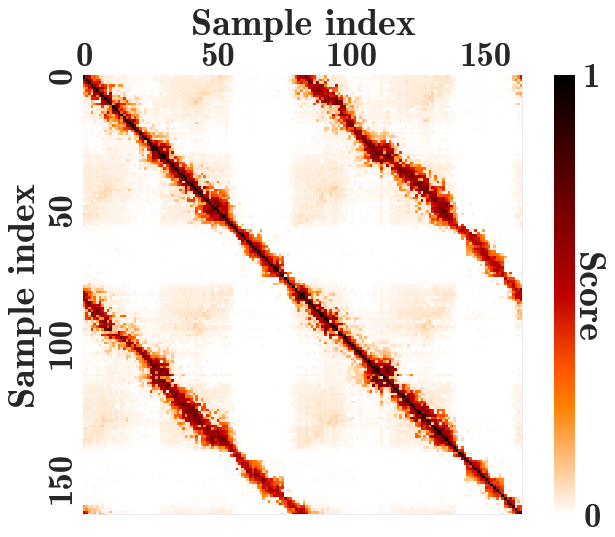
\includegraphics[width=0.32\linewidth]{img/chap_slam/building_scores_matrix.png}}
    %\subfloat[]{\label{fig:forest_scores_matrix}}{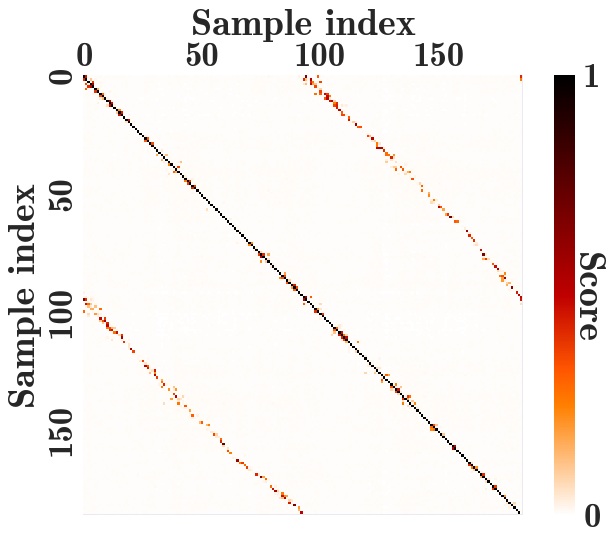
\includegraphics[width=0.32\linewidth]{img/chap_slam/forest_scores_matrix.png}}
    %\subfloat[]{\label{fig:velodyne_scores_matrix}}{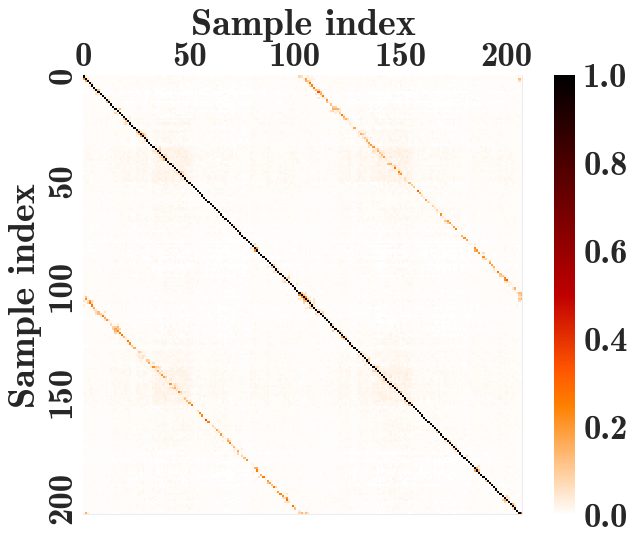
\includegraphics[width=0.32\linewidth]{img/chap_slam/velodyne_scores_matrix.png}} \\

    %\subfloat[]{\label{fig:building_distances_matrix}}{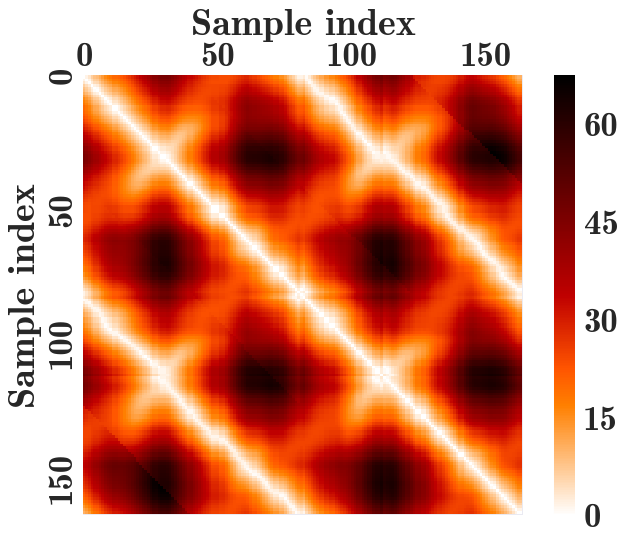
\includegraphics[width=0.32\linewidth]{img/chap_slam/building_distances_matrix.png}}
    %\subfloat[]{\label{fig:forest_distances_matrix}}{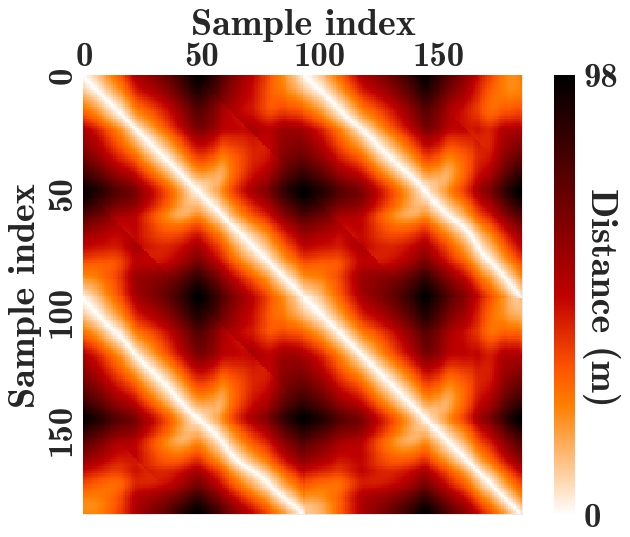
\includegraphics[width=0.32\linewidth]{img/chap_slam/forest_distances_matrix.png}}
    %\subfloat[]{\label{fig:velodyne_distances_matrix}}{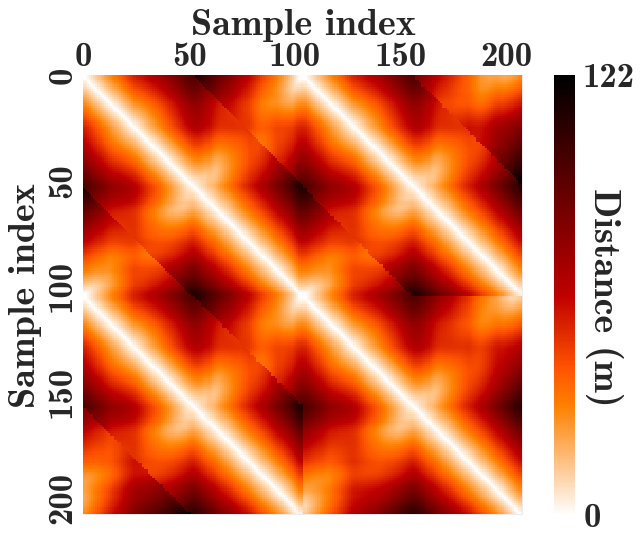
\includegraphics[width=0.32\linewidth]{img/chap_slam/velodyne_distances_matrix.png}} \\

    %\subfloat[]{\label{fig:building_distances_scores_plot}}{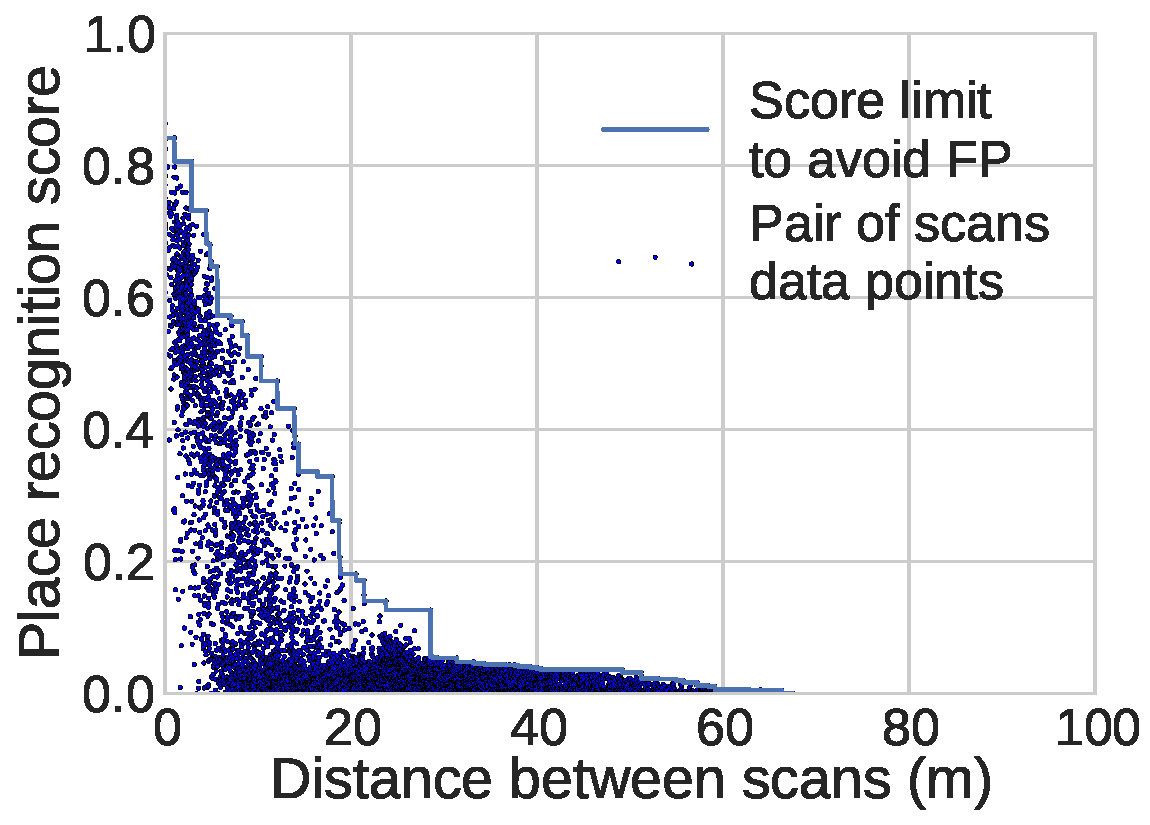
\includegraphics[width=0.32\linewidth]{img/chap_slam/building_distances_scores.pdf}}
    %\subfloat[]{\label{fig:forest_distances_scores_plot}}{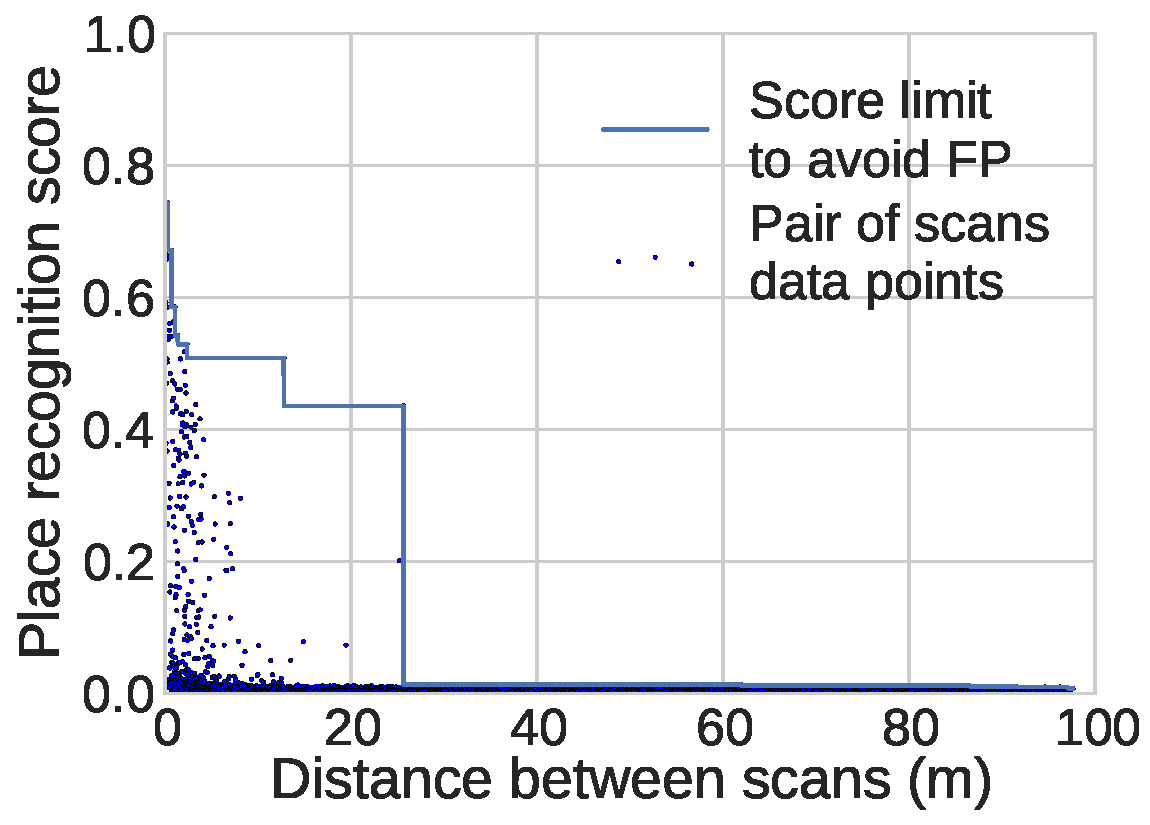
\includegraphics[width=0.32\linewidth]{img/chap_slam/forest_distances_scores.pdf}}
    %\subfloat[]{\label{fig:velodyne_distances_scores_plot}}{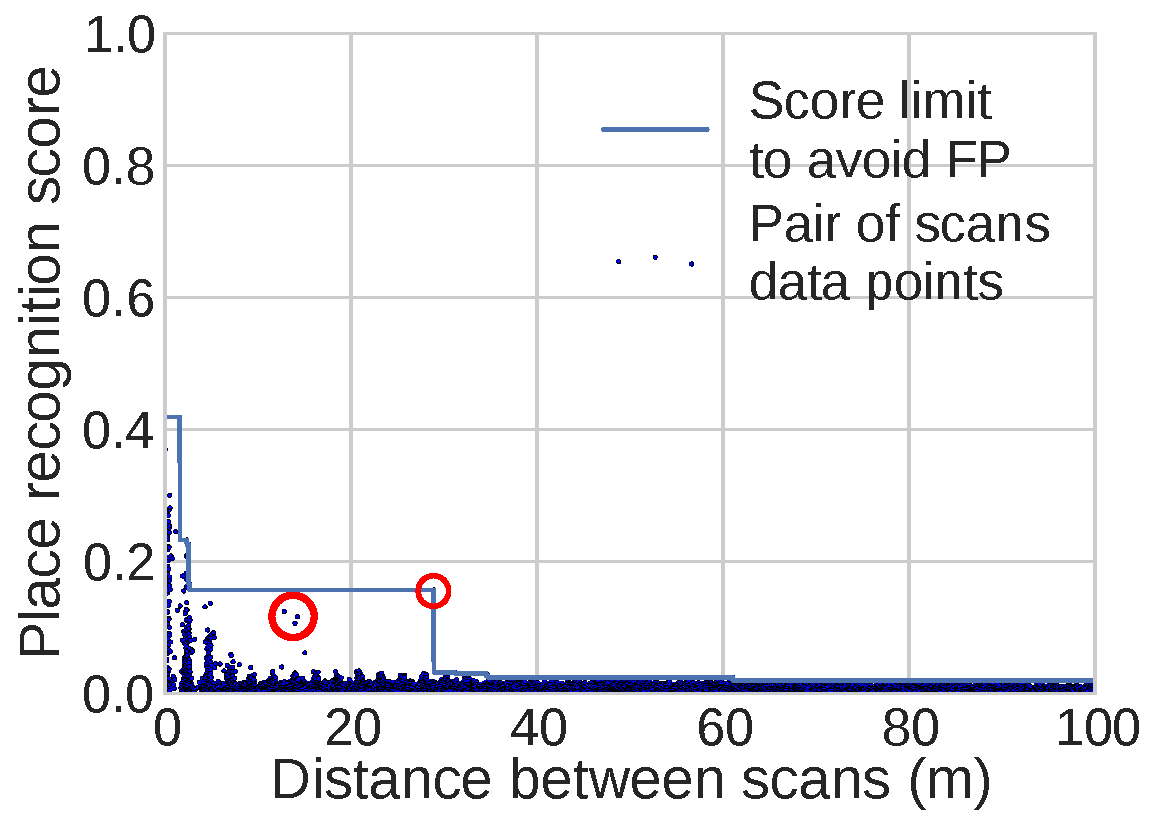
\includegraphics[width=0.32\linewidth]{img/chap_slam/velodyne_distances_scores.pdf}}

    %\subfloat[]{\label{fig:building_recall_plot}}{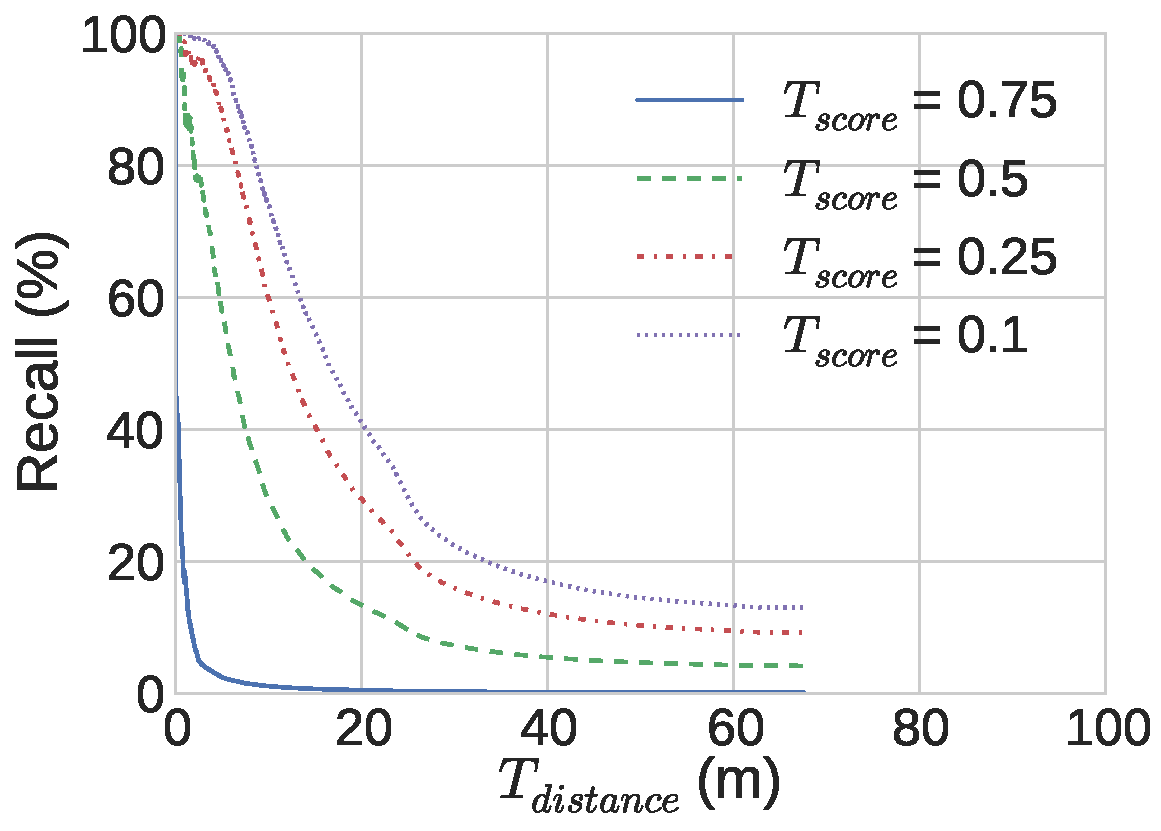
\includegraphics[width=0.32\linewidth]{img/chap_slam/building_recall.pdf}}
    %\subfloat[]{\label{fig:forest_recall_plot}}{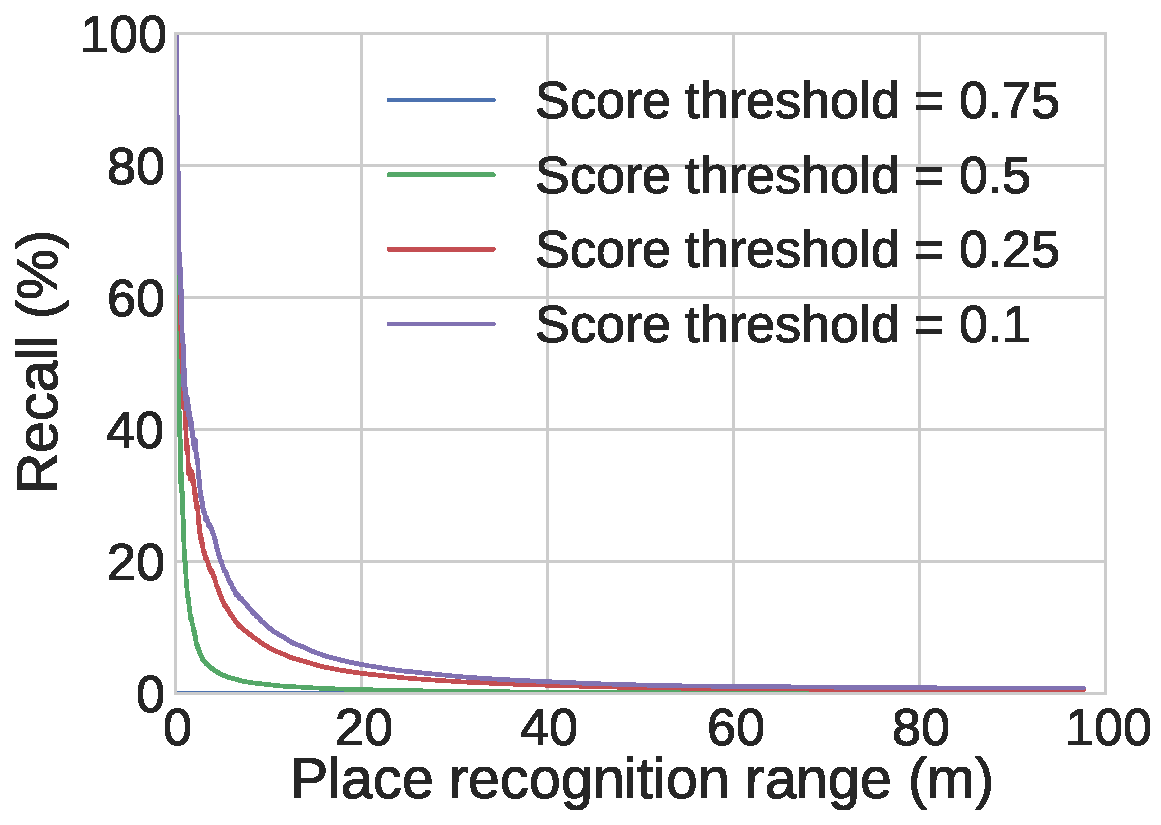
\includegraphics[width=0.32\linewidth]{img/chap_slam/forest_recall.pdf}}
    %\subfloat[]{\label{fig:velodyne_recall_plot}}{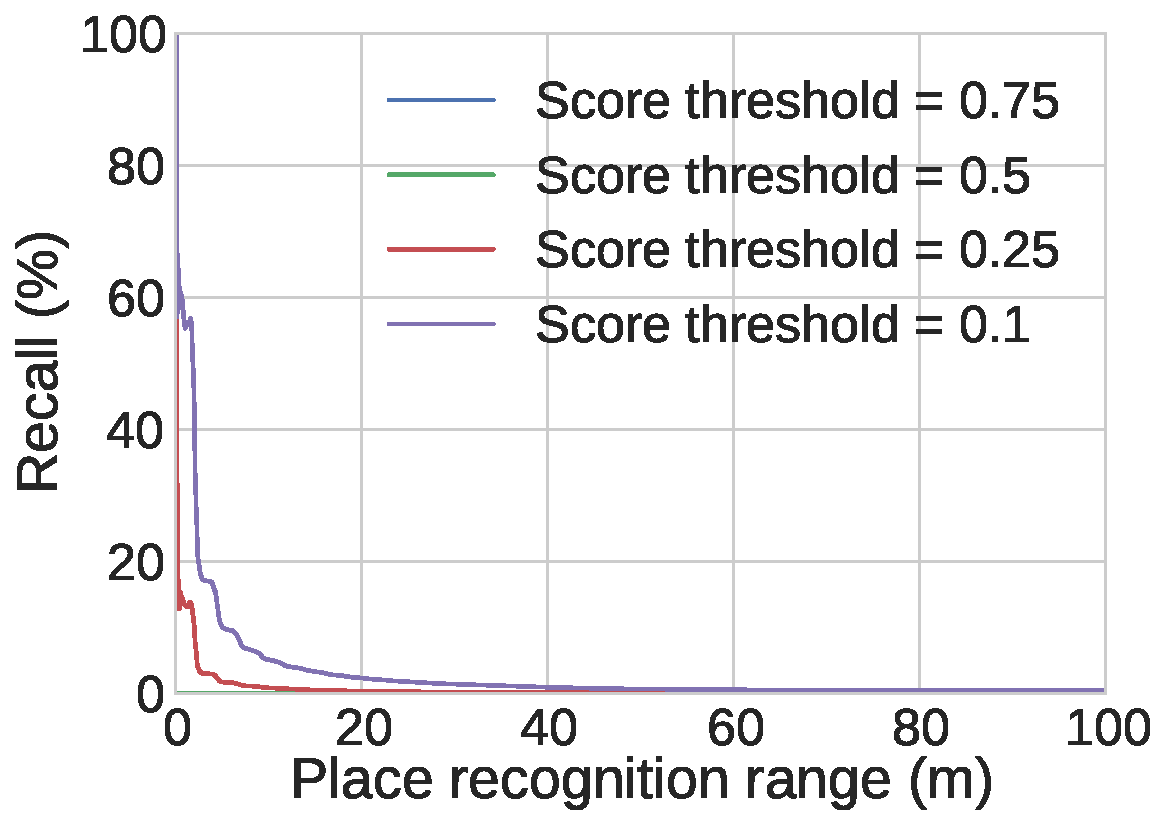
\includegraphics[width=0.32\linewidth]{img/chap_slam/velodyne_recall.pdf}}

    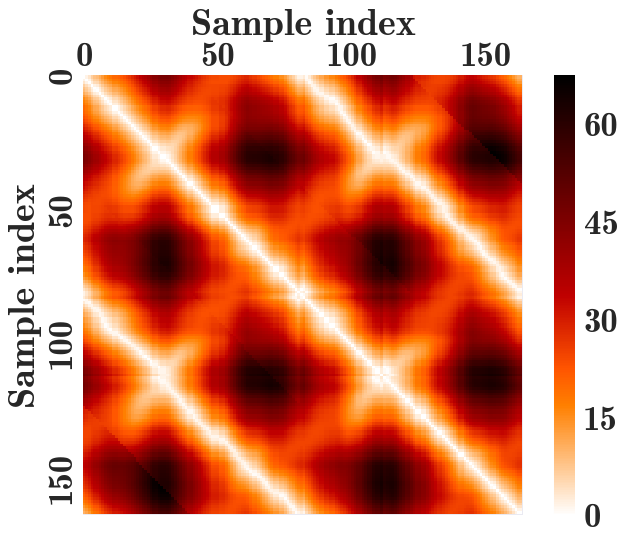
\includegraphics[width=0.32\linewidth]{img/chap_slam/building_distances_matrix.png}
    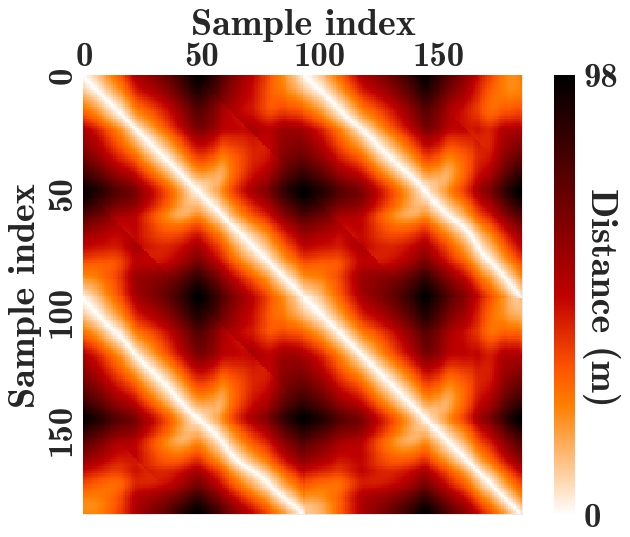
\includegraphics[width=0.32\linewidth]{img/chap_slam/forest_distances_matrix.png}
    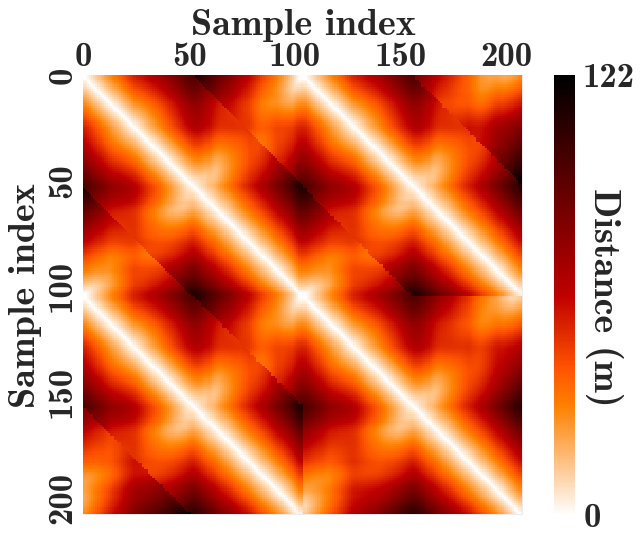
\includegraphics[width=0.32\linewidth]{img/chap_slam/velodyne_distances_matrix.png} \\

    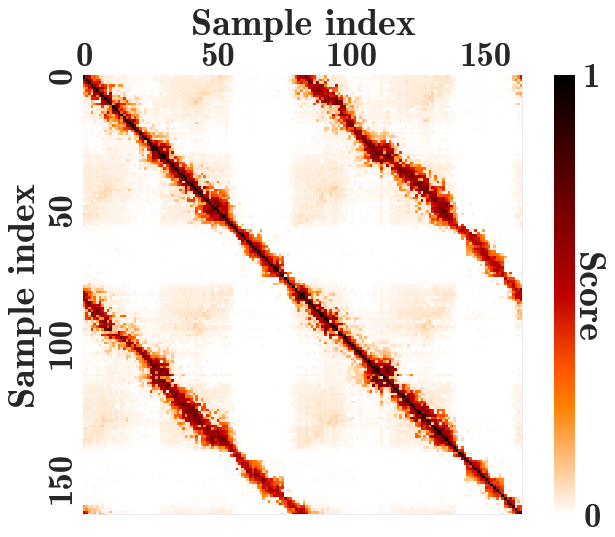
\includegraphics[width=0.32\linewidth]{img/chap_slam/building_scores_matrix.png}
    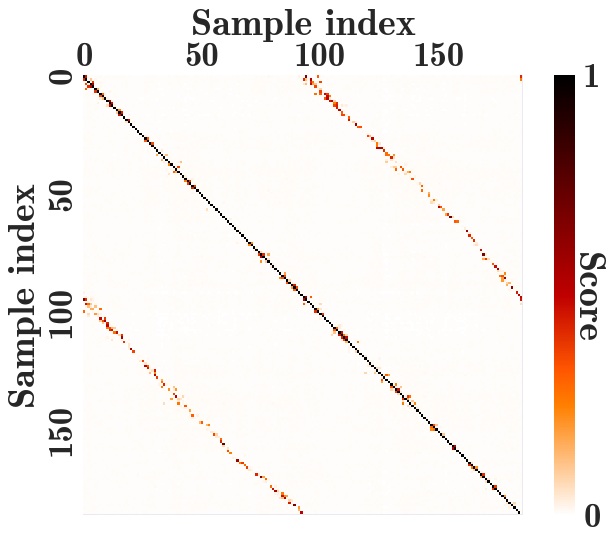
\includegraphics[width=0.32\linewidth]{img/chap_slam/forest_scores_matrix.png}
    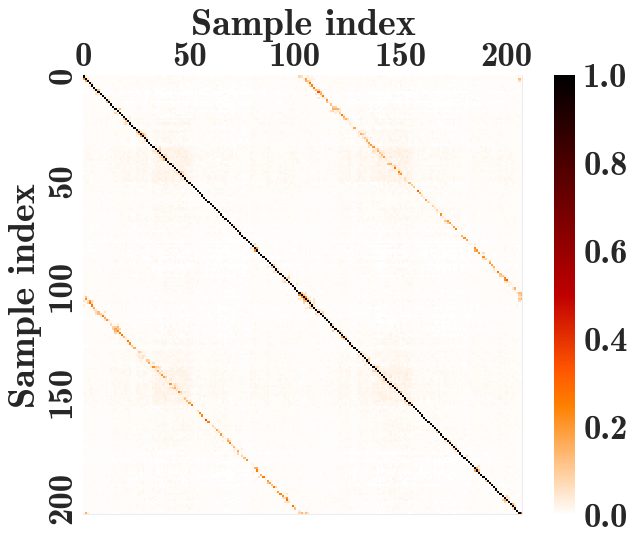
\includegraphics[width=0.32\linewidth]{img/chap_slam/velodyne_scores_matrix.png} \\

    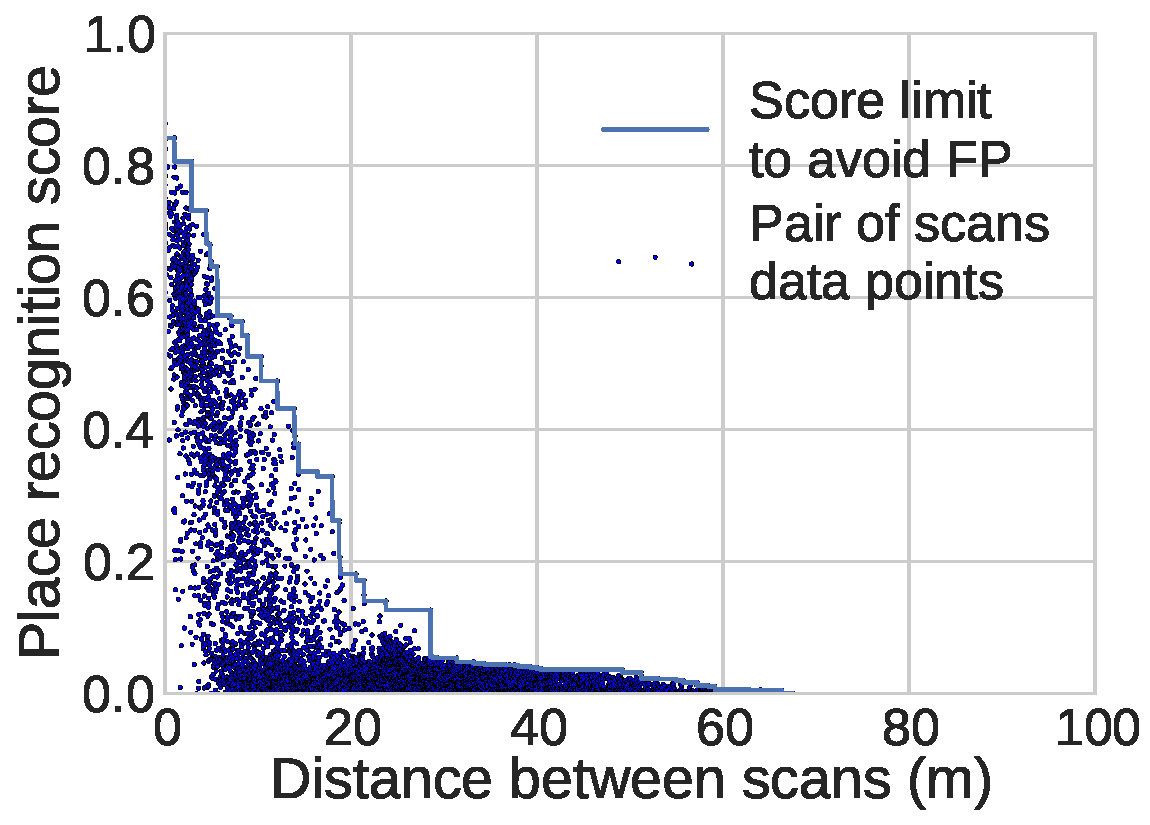
\includegraphics[width=0.32\linewidth]{img/chap_slam/building_distances_scores.pdf}
    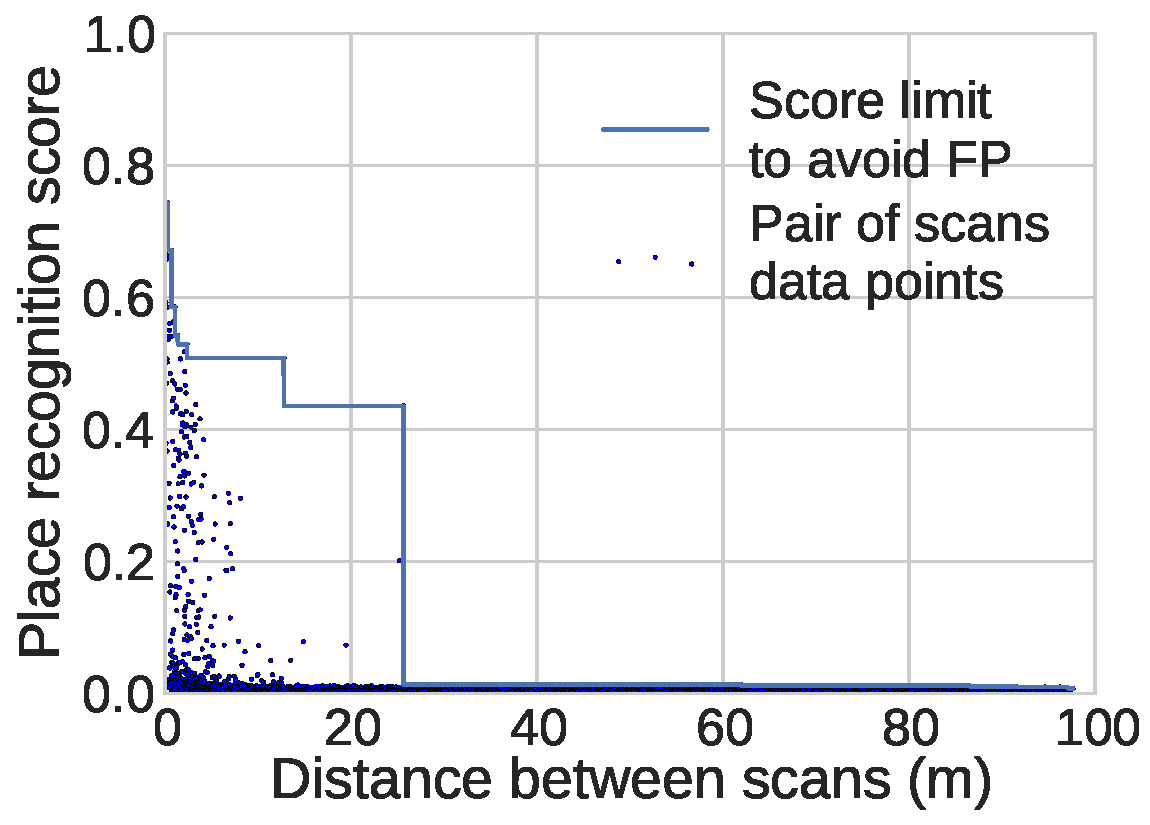
\includegraphics[width=0.32\linewidth]{img/chap_slam/forest_distances_scores.pdf}
    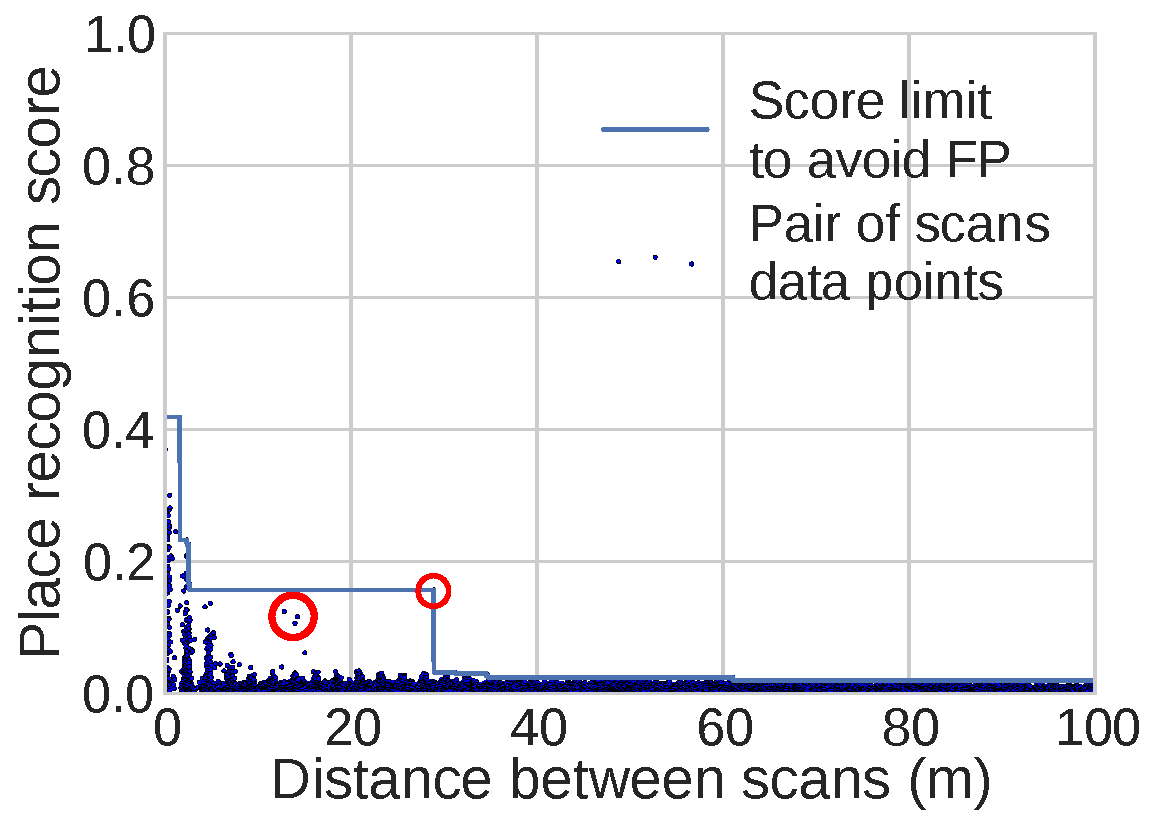
\includegraphics[width=0.32\linewidth]{img/chap_slam/velodyne_distances_scores.pdf} \\

    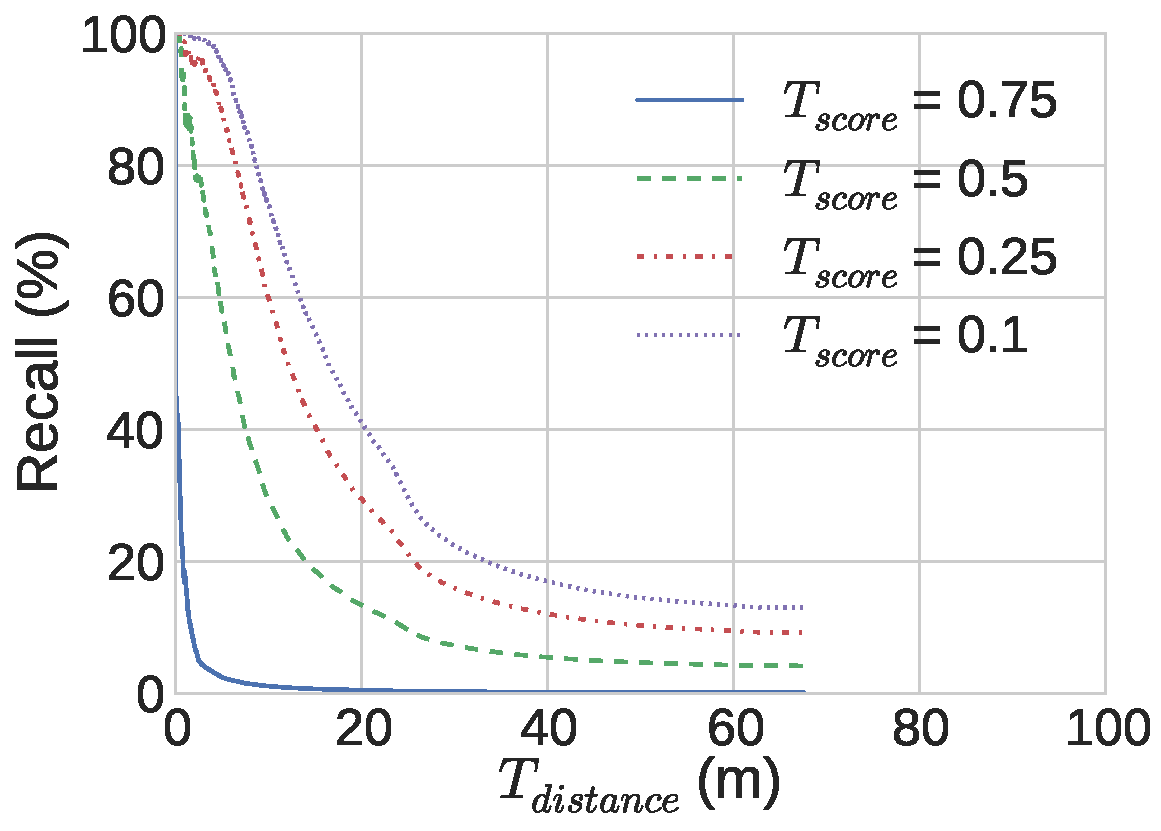
\includegraphics[width=0.32\linewidth]{img/chap_slam/building_recall.pdf}
    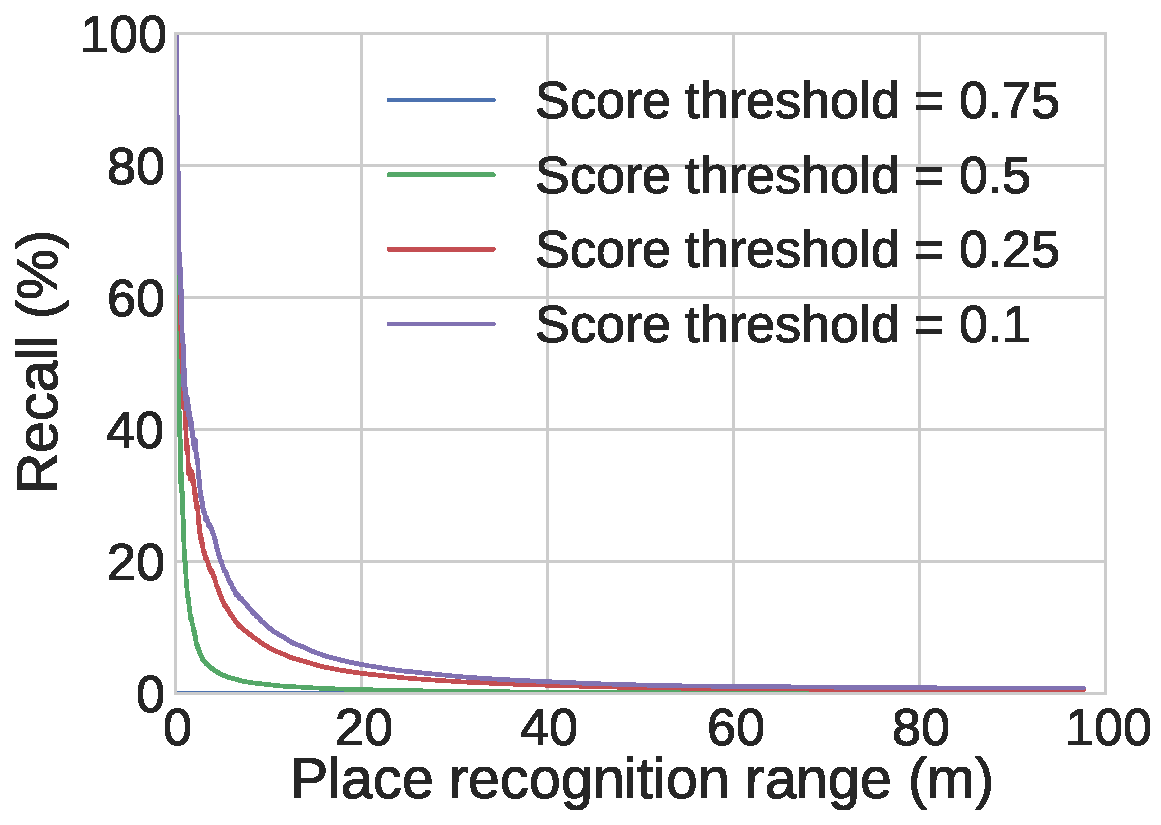
\includegraphics[width=0.32\linewidth]{img/chap_slam/forest_recall.pdf}
    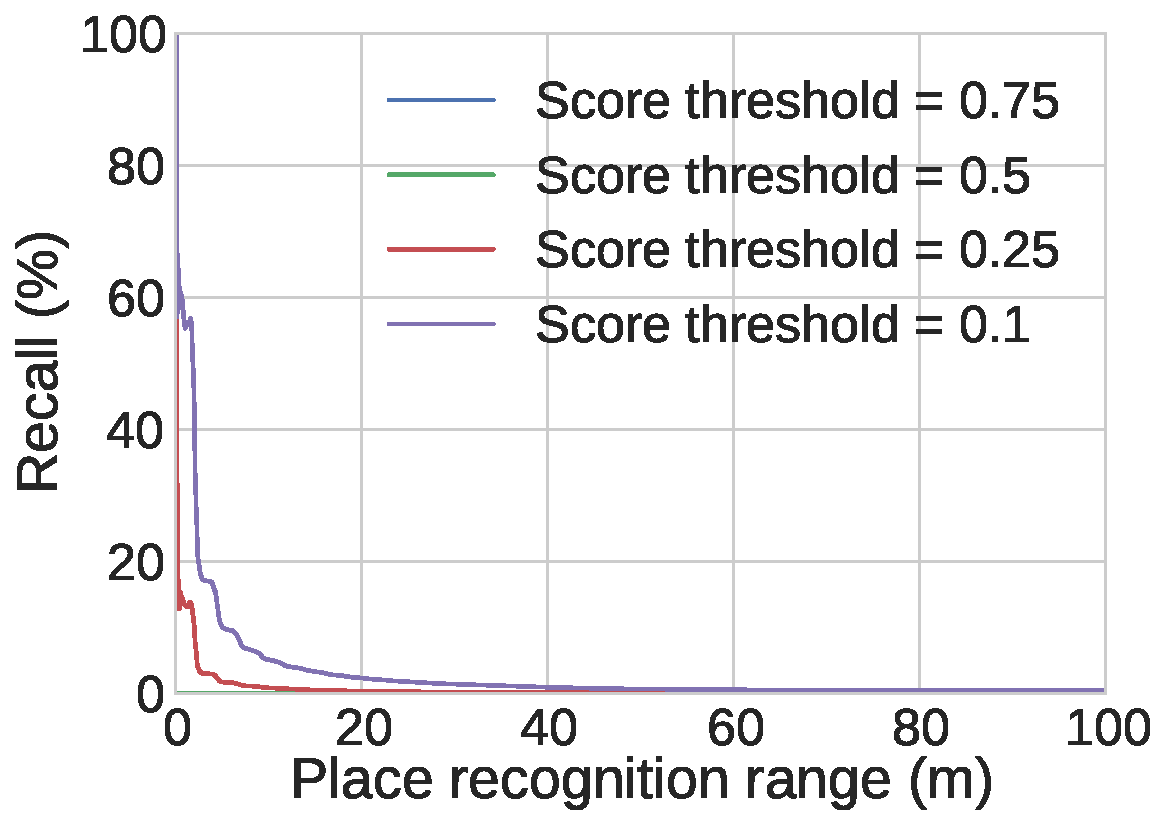
\includegraphics[width=0.32\linewidth]{img/chap_slam/velodyne_recall.pdf}

    \caption[Place recognition results overview for our three datasets.]{Place recognition results overview for our three datasets. \textbf{First column:} The Structured-SICK dataset. \textbf{Second column:} The Unstructured-SICK dataset. \textbf{Third column:} The Unstructured-Velodyne dataset. \textbf{First and second rows:} The matrices of distances and scores, respectively. The axes show the ordered sample indices for both loops sequentially. Consequently, all pairs of scans are represented by a position in the matrices and the color represent the distance between the scans of a pair (first row) and the place recognition algorithm output score (second row). \textbf{Third row:} The association between the distance separating the scans and the score obtained for all scans pairs, as well as the score limit to avoid any \gls*{fp} as function of the distance between the scans. \textbf{Fourth row:} The recall rate as function of the maximum distance (\SI{}{\meter}) between scans to be considered as originating from the same place (place recognition range).} 
    \label{fig:chap_slam_results}
\end{figure}
